
\section{The Calm Before the Storm}

\subsection{Checks, Balances, and Blind Spots}

David signed it.

A single initial. Black ink on cream bond paper.
The final signature on a memo that had already made its way through Risk, Compliance, and Ops.

He set the pen down and exhaled.

\medskip

\begin{figure}[H]
  \centering
  \begin{tikzpicture}[
    node distance=1.8cm and 3cm,
    every node/.style={draw, rounded corners, minimum width=3cm, minimum height=1.5cm, align=center},
    arrow/.style={->, thick}
  ]

    % Nodes
    \node (risk) {Risk\\\small Evaluates exposure\\and model behavior};
    \node (compliance) [right=of risk] {Compliance\\\small Checks mandate\\alignment};
    \node (ops) [right=of compliance] {Ops\\\small Ensures systems,\\routing, execution};
    \node (memo) [below=of compliance] {Memo\\\small Phase II Expansion Approval};
    \node (david) [below=of memo] {David\\\small Final Sign-off};

    % Arrows
    \draw[arrow] (risk) -- (memo);
    \draw[arrow] (compliance) -- (memo);
    \draw[arrow] (ops) -- (memo);
    \draw[arrow] (memo) -- (david);

  \end{tikzpicture}
  \caption{Approval Flow for Phase II Expansion: Risk, Compliance, and Ops all feed into a shared memo reviewed 
  and signed by David.}
\end{figure}

\medskip

\begin{HistoricalSidebar}{Checks and Balances: From Philosophy to Policy}

  The idea of \textbf{checks and balances} — that no single branch or actor should hold unchecked power — traces its 
  roots to the 18th-century political philosopher \textbf{Montesquieu}. In his seminal work, \textit{The Spirit of the 
  Laws} (1748), Montesquieu argued that liberty could only be preserved if power was divided among distinct branches 
  of government: \textit{legislative}, \textit{executive}, and \textit{judicial}. Each branch, he claimed, must be 
  both independent and able to restrain the others.
  
  This principle deeply influenced the \textbf{Founding Fathers of the United States}. Drawing on Montesquieu’s insights, 
  they embedded a system of checks and balances into the U.S. Constitution. Congress could make laws, but the President 
  could veto them. The judiciary could interpret laws, but judges were appointed by the President and confirmed by the 
  Senate. Power, in this design, was fragmented — not to create gridlock, but to force accountability.
  
  \medskip
  
  In modern institutional design --- from financial firms to AI governance --- echoes of this philosophy remain. When it works, 
  no one can act unilaterally. When it fails, it’s often not from the absence of rules, but from the erosion of enforcement, 
  transparency, or communication across those “separate” branches.
  
\end{HistoricalSidebar}

\medskip

The initial run had been a triumph.

Aurora’s Q1 strategy — a volatility-harvest framework with adaptive rebalancing — had done more than 
outperform. It had delivered something far rarer: uncorrelated alpha that actually held.

\medskip

\begin{TechnicalSidebar}{What is Uncorrelated Alpha?}

  In finance, \textbf{alpha} refers to the portion of an investment’s return that exceeds a benchmark — a measure of 
  “skill-based” performance, not just market movement. But not all alpha is created equal.
  
  \medskip
  
  \textbf{Uncorrelated alpha} is the holy grail: returns that are both \textit{above benchmark} and \textit{independent} 
  of broader market swings. This means the strategy isn't just riding a bull market — it’s generating value regardless 
  of whether the S\&P rises or falls.
  
  \medskip
  
  Why does this matter?

  \medskip
  
  \begin{itemize}
    \item For multi-strategy funds and institutional allocators, uncorrelated alpha provides \textbf{diversification 
    at the return level}, not just the asset level.
    \item It helps smooth out portfolio volatility and reduce exposure to systemic risk.
    \item In regulatory or capital-constrained environments, it improves \textbf{risk-adjusted performance without 
    increasing gross exposure}.
  \end{itemize}
  
  \medskip
  
  In Aurora’s case, the Q1 strategy delivered alpha that held steady even as major asset classes whipsawed — not because 
  it avoided volatility, but because it \textit{harvested} it in ways other models couldn't track. That’s what made 
  it valuable.
  
\end{TechnicalSidebar}

\medskip


Tight spreads.
Low drawdown.
Nearly half a billion in clean net gains.

It wasn’t just the money. It was the elegance.
The model moved like a scalpel that sliced volatility, balanced exposure, and skated between the 
rails others hadn’t even mapped.

“Four-eighty,”
\footnote{“Four-eighty” refers to a composite performance metric — typically basis points (bps) of 
return over benchmark — used in internal reviews. In this case, 480 bps (or 4.8\%) above the benchmark 
was considered exceptional, especially for a strategy with modest volatility and low drawdown. 
The reverence wasn’t just for the number, but for what it implied: repeatability.}
 the board had repeated, almost reverently, at the last performance review.
And with it came the question that wasn’t a question:
\textit{If it works here, can it scale across jurisdictions?}

David had hesitated on the inside.
The timing felt wrong. The sync issues were still unresolved. Regulatory variance made synthetic exposure 
a minefield.

``Regulatory variance was the polite term.'', he thought to himself. Then he ran the
the reality through his head.

\medskip

\begin{tcolorbox}[
    enhanced,
    sharp corners,
    boxrule=0pt,
    colback=gray!3,
    borderline west={2pt}{0pt}{gray!60}, % vertical bar on the left
    left=10pt,
    right=10pt,
    top=6pt,
    bottom=6pt,
    width=\linewidth,
    fontupper=\small\itshape
  ]
  In Singapore, swaps had to be cleared.  
  In London, they didn’t — unless the counterparty was EU-based, which meant each trade was a logic tree wrapped in a tax riddle.

  \medskip
  
  In the States, the CFTC still couldn’t decide if their ruling applied to structures involving forward-settling derivatives nested inside funds-of-funds —  
  and meanwhile, the SEC pretended like that kind of exposure didn’t even exist.

  \medskip
  
  
  It wasn’t just red tape.  
  It was contradictory compliance built on different definitions of the word “exposure.”

  \medskip
  
  
  In New York, a product could pass muster as a hedged position.  
  In Zurich, the same position was flagged as synthetic leverage.  
  In Tokyo, they didn’t even have a category for it — which made disclosure discretionary.

  \medskip
  
  And then there were the audit trails.  
  Europe required transparency portals.  
  The U.S. only cared if it hit GAAP.  
  Hong Kong? They liked their risk buried — just so long as the net exposure stayed under 2.5x assets.
\end{tcolorbox}
  
\medskip

David leaned back in his chair.

It wasn’t the regulators he feared.
It was the gaps between them.
Because that’s where arbitrage lived.

\medskip

\begin{TechnicalSidebar}{Arbitrage --- The Riskless Profit That Isn’t (Always)}

    \textbf{Arbitrage} is the financial equivalent of spotting a \$20 bill lying between two 
    vending machines, and picking it up before someone else does.

\medskip
    
    At its core, \textbf{arbitrage} means exploiting price differences for the \textbf{same} 
    asset across \textbf{different} markets to make a profit with *no net risk*.

\medskip
    
    \textbf{Classic Example:}  
    You see gold priced at \$1,800/oz in London, but \$1,805/oz in New York.  
    If you can buy in London and sell in New York fast enough (before prices realign), you pocket \$5/oz.  
    No guesswork. No forecasting. Just pure timing.

\medskip
    
    \textbf{Common Real-World Variants:}

\medskip

    \begin{itemize}
      \item \textbf{Currency Arbitrage:}  
      EUR/USD is trading at 1.100 in one market and 1.101 elsewhere. A well-structured trade nets 
      the 0.001 spread.
    
      \item \textbf{Retail Arbitrage:}  
      Buy limited-edition sneakers for \$150 at a local store. Resell them for \$300 online. The asset 
      is physical, but the arbitrage logic is identical.
    
      \item \textbf{Triangular Arbitrage (Forex):}  
      Convert USD to EUR, then EUR to GBP, then GBP back to USD; and if done through certain routes 
      with small inefficiencies, you end up with more USD than you started with. 
    
      \item \textbf{Regulatory Arbitrage:}  
      A financial product that's illegal in one country but legal in another might be structured offshore. 
      This isn't strictly price arbitrage. It's rules arbitrage.
    \end{itemize}
    
\medskip
    
    \textbf{Why It Matters in Finance:}  
    Large firms and hedge funds build entire platforms to detect and execute arbitrage opportunities in 
    milliseconds. But:
    
    \begin{quote}
      Arbitrage only works when others haven't noticed it yet. Once they do, the price gap disappears.
    \end{quote}
    
    \textbf{Modern Twist:}  
    In today’s market, arbitrage isn't just about price. It's also about \textit{latency}, 
    \textit{jurisdiction}, and \textit{legal interpretation}.  
    This is why synthetic instruments across borders become dangerous:  
    You're not just arbitraging price.  
    You're arbitraging the space between regulators.
    
\end{TechnicalSidebar}

\medskip

The question echoed again in his head:

\begin{quote}
    If it works here, can it scale across jurisdictions?
\end{quote}

``Sure.'' he thought to himself. 

He could hear the slick, sardonic, half-mocking voice in his head: ``If you didn’t mind rewriting 
the same engine three times... and,
if you didn’t mind time-zone compliance teams who didn’t speak the same risk language...
And, if you didn’t mind the clients pretending they didn’t notice the mismatch as long 
as the returns printed''

He knew the answer wasn’t ``yes'' and it wasn’t ``no'' either.

The answer was... 
\begin{quote}
    \centering
    it depends.
\end{quote}

The answer is always ``it depends.''

That's the way that Hart liked it.

``This isn’t just performance,'' he’d said. ``It’s a narrative. Aurora’s running headlines. Investors love 
velocity.''

And it was true that they were moving fast.
Too fast for David’s comfort.
But somehow, impossibly, they kept pulling it off.

So Phase II was approved:
\textbf{Cross-jurisdictional execution}, routed through Arcadia’s London desk.

\medskip

\begin{HistoricalSidebar}{Cross-Jurisdictional Execution: Speed, Fragmentation, and Shadows}

  Cross-jurisdictional execution — the routing of trades across international desks to exploit 
  latency, regulatory 
  arbitrage, or access — has long been both a competitive advantage and a systemic blind spot.

  \medskip
  
  In the early 2000s, hedge funds began routing European equity trades through U.S. dark pools 
  to avoid MiFID 
  restrictions. Conversely, U.S. desks routed through London to exploit favorable derivatives 
  treatment. The 2010 
  Flash Crash revealed how fragmented venues, spread across time zones and compliance domains, 
  could react with 
  incoherent logic in milliseconds.

  \medskip
  
  By 2015, major asset managers were running execution algorithms that spanned Tokyo, London, 
  Frankfurt, and New 
  York. Compliance regimes couldn’t keep up.

  \medskip
  
  Cross-border desks brought speed and flexibility — especially in synthetic instruments like 
  CFDs, TRSs, and 
  offshore swaps. But they also brought latency mismatches, disconnected kill switches, and 
  jurisdictional confusion 
  in crisis response.

  \medskip
  
  After Archegos (2021), regulators flagged how synthetic positions spread across prime brokers in 
  different legal 
  systems could accumulate unmonitored. But enforcement lagged.

  \medskip
  
  \textbf{The promise:} optimal routing, alpha capture, and 24/6 liquidity.

  \medskip

  \textbf{The risk:} fragmented oversight, circular hedging, and response delays measured in billions.
  
\end{HistoricalSidebar}

\medskip



\subsection{Elastic Exposure, Rigid Assumptions}

The pitch was simple:
Tighter latency on European venues.
Flexible regulatory treatment of synthetic instruments.
Speed, at scale.

The risk?
\textit{Contained.} At least, according to the memo he just signed.

He didn’t love the language.

\begin{itemize}
    \item ``Elastic notional synthesis.'' 
    \item ``Latency-sliced positioning.'' 
    \item ``Behavior-aware hedging.''
\end{itemize}

It read like a PowerPoint built for people who liked the sound of algorithms more than the 
feel of them.

But it wasn’t his call anymore.

David had scoped the model with his team, built it to breathe in narrow bands, and calibrated it for edge 
cases and gentle undulations.
It wasn’t built for speed.
It was built for resilience.

He’d insisted on constraints early — not because they looked good in a compliance deck, but because 
he knew what happened to models that grew too fast without discipline. They didn’t crash noisily. 
They drifted. They wandered from their training boundaries, mistaking correlation for cause, 
extrapolating patterns from noise.

So he made the team do it the hard way.
Stress it. Squeeze it. Make it learn how to be wrong — gently.

The model wasn’t optimized to chase alpha in every tick.
It was built to survive the whiplash.
To know when to hold, when to hedge, and when to stop trusting its own instincts.

He’d run simulations that didn’t reward success — they penalized overconfidence.
He made sure the confidence intervals were wide where they needed to be, and shallow where assumptions 
got thin.

It didn’t always win fast.
But it didn’t overfit. It didn’t hallucinate. It didn’t panic.

He hadn’t built a sniper.
He’d built a climber. One that knew the terrain would shift beneath it — and that staying upright mattered 
more than moving first.

\medskip

\begin{TechnicalSidebar}{Why Machine Learning Models Must Be Continuously Trained}

  Machine learning models are not static assets.  
  They are probabilistic approximators—trained not to be \textit{correct}, but to be 
  \textit{informationally relevant} to the distribution they’ve seen.
  
  \medskip
  
  \textbf{But that distribution moves.}

  \medskip
  
  In trading systems, this is called \textit{non-stationarity}. In ML theory, it's 
  \textit{distributional drift}. In practical terms:  
  what worked yesterday might fail quietly tomorrow.
  
  \medskip
  
  A model trained on old market conditions may:

  \medskip
  
  \begin{itemize}
    \item Suppress signals it now considers noise
    \item Misclassify valid anomalies as benign
    \item Overfit to structural patterns that no longer exist
  \end{itemize}

  \medskip
  
  Worse: without retraining, the confidence scores remain high—even as accuracy degrades.  
  This is the most dangerous form of model failure: \textbf{not silent, but self-assured.}
  
  \medskip
  
  \textbf{Continuous retraining} isn’t a nice-to-have. It’s survival.  

  \medskip

  It requires:

  \medskip
  
  \begin{itemize}
    \item Streaming pipelines for ingesting new data
    \item Validation infrastructure that can reweight on the fly
    \item Human oversight for flagging edge-case drift before it calcifies into error
  \end{itemize}

  \medskip
  
  In theory, all models degrade.  
  In practice, only the ones that get updated stay useful.
  
\end{TechnicalSidebar}

\medskip

\begin{HistoricalSidebar}{The Zillow Collapse}

  \textbf{In 2021, Zillow learned the hard way what happens when a model goes stale.}

  \medskip
  
  At the heart of its failure was the \textit{Zestimate} algorithm—a proprietary machine learning 
  model built to 
  predict home values.  
  Zillow wasn't just using it for browsing anymore. They were using it to buy real houses.
  
  \medskip
  
  \textbf{The bet:} if their model was accurate within a narrow margin, they could algorithmically 
  flip properties at scale.  

  \medskip

  \textbf{The reality:} the model was trained on historical data, in a market that was changing 
  faster than the 
  retraining loop could adapt.
  
  \medskip
  
  \textbf{What went wrong?}

  \medskip
  
  \begin{itemize}
    \item \textbf{Feedback lag:} The model relied on past sale data. But in a hot market, sale prices 
    lagged real-time 
    demand shifts.
    \item \textbf{Distributional drift:} Market dynamics changed post-COVID—inventory shocks, urban 
    flight, remote 
    work—but the model assumed stationarity.
    \item \textbf{Overconfidence:} As model performance degraded, Zillow continued scaling up 
    purchases—trusting 
    predictions that no longer reflected reality.
  \end{itemize}

  \medskip
  
  \textbf{The result:}  Zillow wrote down over \$500 million in losses, liquidated its inventory, and 
  laid off 25\% of 
  its workforce.
  
  \medskip
  
  The lesson wasn’t just about real estate.  
  It was about models—and what happens when leadership mistakes \textit{confidence} for \textit{validity}.
  
  Zillow didn’t just misprice homes.  
  They operationalized a model faster than they could audit it.
  
  And the market noticed.
  
\end{HistoricalSidebar}

\medskip

\begin{figure}[H]
  \centering
  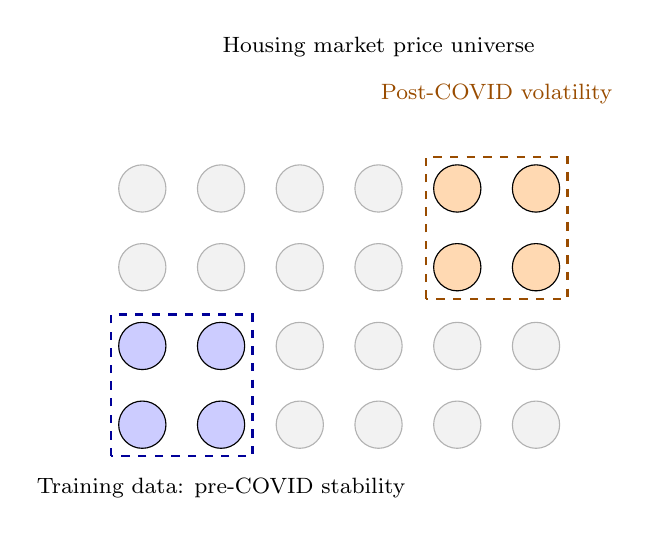
\begin{tikzpicture}[
      stable/.style={circle, draw=black, fill=blue!20, minimum size=0.6cm},
      covid/.style={circle, draw=black, fill=orange!30, minimum size=0.6cm},
      neutral/.style={circle, draw=black!30, fill=gray!10, minimum size=0.6cm},
      every node/.style={font=\scriptsize}
  ]
  
  % Grid layout (6x4)
  \foreach \x in {0,1,2,3,4,5} {
      \foreach \y in {0,1,2,3} {
          \node[neutral] (n\x\y) at (\x, \y) {};
      }
  }

  % Training data for stable market (left 2x2)
  \foreach \x in {0,1} {
      \foreach \y in {0,1} {
          \node[stable] at (\x, \y) {};
      }
  }

  % New dynamics during COVID (right 2x2)
  \foreach \x in {4,5} {
      \foreach \y in {2,3} {
          \node[covid] at (\x, \y) {};
      }
  }

  % Labels
  \node[align=left, font=\footnotesize] at (1, -0.8) {Training data: pre-COVID stability};
  \node[align=left, font=\footnotesize, text=orange!60!black] at (4.5, 4.2) {Post-COVID volatility};
  \node[align=left, font=\footnotesize] at (3, 4.8) {Housing market price universe};

  \draw[dashed, thick, blue!60!black] (-0.4, -0.4) rectangle (1.4, 1.4);
  \draw[dashed, thick, orange!60!black] (3.6, 1.6) rectangle (5.4, 3.4);

  \end{tikzpicture}
  \caption{Model Failure from Distributional Drift: Zillow’s prediction engine trained on pre-COVID stability (blue), but volatility emerged in unmodeled housing zones (orange).}
\end{figure}








\subsection{The Architecture of Execution}

Across the floor, terminals glowed in muted hues.  The espresso machine hissed like a stress valve.  It was morning in 
New York, and London was already deep into the session.

Kayla, from execution strategy, leaned in through the open doorframe.

\medskip

\begin{TechnicalSidebar}{What Is Execution Strategy?}

  \textbf{Execution strategy} is the set of methods, rules, and tools used to convert a trading idea into actual trades — 
  as efficiently and cost-effectively as possible.
  
  \medskip
  
  In modern markets, the challenge isn’t just \textit{what} to buy or sell. It’s \textit{how}.
  
  \medskip
  
  An execution strategist focuses on:
  
  \begin{itemize}
    \item \textbf{Minimizing slippage:} ensuring trades don’t move the market too much.
    \item \textbf{Timing and fragmentation:} deciding which venues to hit, in what sequence, and at what speed.
    \item \textbf{Adaptive routing:} choosing real-time paths through exchanges, dark pools, and synthetic liquidity 
    providers.
    \item \textbf{Managing execution risk:} monitoring fills, latency, and adverse selection.
  \end{itemize}
  
  \medskip
  
  At the institutional level, execution strategy blends quantitative modeling with market microstructure expertise 
  because even a perfect model can underperform if executed poorly.
  
\end{TechnicalSidebar}

\medskip

“London’s cleared for rollout,” she said, stopping a few feet behind him. “I verified that we’re pre-positioned 
across the LSE, Cboe Europe, and Turquoise venues.”

\medskip

\begin{TechnicalSidebar}{What is Pre-Positioning?}

  \textbf{Pre-positioning} refers to the strategic placement of capital, orders, or algorithmic models across multiple 
  trading venues \textit{before} execution begins.  
  It ensures that when the market moves — or when a system is triggered — the infrastructure is already in place to 
  respond instantly.

  \medskip

  In high-frequency or cross-jurisdictional trading, milliseconds matter.  
  Pre-positioning reduces latency and slippage by eliminating the need to request access or deploy logic in real time.

  \medskip

  It can include:

  \begin{itemize}
    \item \textbf{Capital allocation:} Ensuring margin or collateral is already posted at multiple exchanges.
    \item \textbf{Order scaffolding:} Pre-loaded orders or algorithms waiting for live market triggers.
    \item \textbf{Model mirroring:} Synchronizing trading models across geographies (e.g., New York, London, Singapore) 
    for rapid parallel execution.
    \item \textbf{Infrastructure warm-up:} Keeping compute resources active and primed to route orders.
  \end{itemize}

  \medskip

  In Kayla’s update, “pre-positioned across three venues” means Aurora’s systems had already staged trades and routing 
  logic in advance.  
  The model could engage immediately — no warm-up, no requests, just execution. It’s how you move fast in markets that 
  punish hesitation.

\end{TechnicalSidebar}

\medskip

David didn’t turn around. He just nodded with a nod that said ``yes'', but thought ``God, I hope so''.

Because even now, even after the test clears and the checklist ticks, the reel is still playing in his head — 
back to the room where they’d made the call.

They’d been in Geneva, two weeks before rollout. A whiteboard full of venue maps, latency curves, and fill 
curves was still half-visible behind the reflection of the window.

"Three tiers?" someone had asked.
"No. We pick three names we trust," David had said.
"LSE, Cboe Europe, Turquoise. Between them, you cover core liquidity, synthetic rerouting, and dark overlays."

"But we could split across eight—"
"—and get eight different risk profiles," he’d cut in.

He remembered tapping the board with the back of his pen.
“We’re not building an experiment. We’re building a highway.”

He remembered thinking: venues are like roads.
You don’t just care if they’re open. You care what kind of traffic they carry.

\begin{itemize}
\item \textbf{LSE} was legacy. Deep books, predictable behavior, slower to stress. Like a stable old artery through the city.
\item \textbf{Cboe Europe} had agility — tighter spreads, cross-product hooks, and better slippage handling in high-turnover names.
\item \textbf{Turquoise} was the wildcard: low visibility, better dark fill ratios, optional midpoint matching.
\end{itemize}

Each venue was its own ecosystem, and its own style of liquidity.
They weren’t just execution pipes. They were behavioral signatures.

And choosing them meant choosing the kind of failure you were willing to have.

Back then, he had said it out loud:
"If it breaks, I’d rather break predictably. I’d rather break where I know who else is in the water."

Now, standing at the edge of deployment, David thought through the breakpoints — not just abstract risk, but personality under pressure.

\begin{itemize}
\item \textbf{LSE}, he knew, would crack slowly.
It wouldn’t collapse; it would glide. Liquidity would thin at the open, auctions would widen, and fills would start arriving with a time lag you could mistake for latency — until it wasn’t.
The danger wasn’t speed. It was drift. You’d still be trading, still seeing prints. You just wouldn’t realize you were the only one left on the other side of the book until it was too late.

\item \textbf{Cboe}, by contrast, would snap like a carbon fiber rod.
It was efficient, until it wasn’t. The algo hooks would overreact. Internalizers would front-run their own signals. One volatility spike and the venue’s adaptive behavior would cross the line from tactical to chaotic.
David could already picture it: the logs would show perfect logic — just executed faster than humans could adjust.
The failure wouldn’t be from slowness. It would be from trusting the machine to pause when it should pivot.

\item \textbf{Turquoise} was a different beast.
Turquoise didn’t break; it vanished. One moment it was your stealth leg — matching size without signaling — and the next it was a black hole.
No fills. No errors. Just silence.
The danger wasn’t visible. It was epistemic.
You couldn’t manage what you couldn’t prove was happening. And that was the point: dark liquidity never screamed. It ghosted.
\end{itemize}

So yes — they were the best bets.
But even the best roads had blind curves.
And now he wondered, not for the first time, if they’d mapped enough of the terrain...
or just memorized the routes that hadn’t crashed yet.

Now, standing at the desk, he wished he’d spent more time modeling what happened when they all broke 
the same way.

He could still hear his own voice from Geneva, calm and confident:
\textit{"We’re not building an experiment."}

But now, watching the screen, that’s exactly what it felt like.

An experiment they couldn’t rewind.
And a test that wasn’t finished until it failed.

\medskip

\begin{table}[H]
    \centering
    \caption*{\textbf{Venue Selection Matrix: Geneva Rollout Strategy}}
    \begin{tabular}{|l|c|p{8cm}|}
    \hline
    \textbf{Venue} & \textbf{Selected} & \textbf{Reason} \\
    \hline
    \textbf{LSE (London Stock Exchange)} & \checkmark & Deep order books, legacy reliability, lower volatility under stress. Behaves like a backbone route — stable and predictable. \\
    \hline
    \textbf{Cboe Europe} & \checkmark & Strong routing logic, tight spreads, adaptive during high turnover. Good fill quality in volatile names. \\
    \hline
    \textbf{Turquoise} & \checkmark & Access to dark liquidity, high midpoint match ratios. Used for stealth size placement. \\
    \hline
    \textbf{Euronext} & $\times$ & Less predictable during cross-venue slippage. Increased latency on synthetic reroute pathways. \\
    \hline
    \textbf{Xetra} & $\times$ & Clean structure but overly rigid auction boundaries — not ideal for dynamic strategy rebalancing. \\
    \hline
    \textbf{Chi-X Europe} & $\times$ & Good for speed but poor dark fill consistency. Too prone to ghost liquidity and spoofing artifacts. \\
    \hline
    \textbf{SIX Swiss Exchange} & $\times$ & Limited cross-product integration and insufficient depth in key instruments during Asia overlap hours. \\
    \hline
    \end{tabular}
\end{table}














\subsection{Staggered Ignition}

David didn’t turn. “All equity, as expected?”

“Cash and ETF blocks only,” she confirmed. “Derivs stay in Chicago, FX still sleeps until New York opens. 
Core inventory’s clean and loaded.”

The thesis was: \textbf{staggered ignition.}

\begin{itemize}
\item \textbf{Cash equity first}, for clarity and control.
\item \textbf{ETF blocks} second, to scale without drawing attention.
\item \textbf{Derivatives deferred}, to avoid triggering the machines.
\item \textbf{FX last}, because currency would follow — not lead — the story.
\end{itemize}

He gave a fractional nod that looked like acceptance but felt like interrogation.

Because in his head, the clock wound backward again... to the allocation meetings.
To the diagrams.
To the models they thought were conservative enough.

\textit{That meeting had happened in a glass-walled room with the clocks muted.}

They’d gone line by line through the flowbook.

David stared at the blotchy matrix on the screen — heatmap red creeping outward like a rash.

“Cash leads?”

The question hung in his mind before he even spoke it aloud. Not because he didn’t know the answer — but because saying it would make it real. The kind of real that burned bridges you might need later.

He already knew the answer.

Yes — equities first.

Stocks were the low-hanging fruit. Liquid, visible, brutally honest. You could watch them tick down in real time like a dying pulse. No need for model recalibration or custom pricing logic — just click, confirm, sell. Gone.

Faster to price.

Everyone in the market agreed, whether they admitted it or not. Equities told you the truth quickly. Sometimes too quickly. Bonds took negotiation. Derivatives? A minefield. Private investments? Deadweight in a crisis. But stocks… stocks could bleed for you on command.

Easier to throttle.

He could trim the book in layers — 5\%, 10\%, 15\% — and still pretend it was strategy, not surrender. No fire sale headlines, no panic in the execution logs. Just controlled bleeding. He could even tag it as "rebalancing" if anyone asked.

David tapped the side of his keyboard, not typing — just thinking.

Cash wasn’t just about liquidity anymore. It was posture. It was signal. And when the tide turned — if it turned — having cash meant you got to choose who drowned.

But first, you had to be willing to pull the lever.

\medskip

\begin{TechnicalSidebar}{Cash Leads: Why Equities Fire First}

    In multi-asset execution strategies, the term \textbf{``cash leads''} refers to sequencing logic where 
    \textbf{cash equities} (stocks) are executed first — before related derivatives or hedges — to anchor the position.
    
    \medskip
    
    This is often done for the following reasons:

    \medskip
    
    \begin{itemize}
      \item \textbf{Price Certainty:}  
      Cash equities are directly observable and more liquid than their derivative counterparts. They can be priced and filled more quickly, especially in high-volume venues.
    
      \item \textbf{Throttling Simplicity:}  
      Cash orders can be easily throttled or paused mid-stream without triggering complex chain effects in hedge books or synthetic baskets.
    
      \item \textbf{Anchor Pricing:}  
      Executing the cash leg first sets a reference price for any subsequent derivative trades (e.g., futures, options, swaps), reducing slippage risk in delta-neutral or cross-asset strategies.
    
      \item \textbf{Latency Management:}  
      In fragmented markets (e.g., US equities), smart order routers can aggressively sweep or passively rest across venues with more consistent latency than in synthetic or OTC instruments.
    \end{itemize}
    
    \medskip
    
    \textbf{In Plain Terms:}  
    Firing the cash leg first is like placing the stable piece on a chessboard — it anchors the strategy.  
    Everything else (hedges, derivatives, overlays) reacts to that anchor.  
    It’s not just about speed.  
    It’s about control.
    
\end{TechnicalSidebar}

\medskip


“And ETFs?”

The thought surfaced before the words. He didn’t ask the question out loud — not yet. It was a mental check, a second pass through the triage list. He needed to know how deep the floor was before stepping onto it.

They weren’t pretty this early. Illiquid, wide spreads, and the pre-market tape looked more like a drunk algorithm’s confession than real price discovery. But still... safer than futures.

They’re shallow pre-open… but safer than futures.

Futures were faster, yes — brutal and immediate — but they cut both ways. A little slippage and the whole desk would wear the mark-to-market loss like a scar. One bad fill and compliance would be at his door with a chart, a timestamp, and a question he couldn’t afford to answer truthfully.

No mark-to-market shock if we get slippage.

That was the game now: not avoiding risk, but hiding it just long enough to reposition. With ETFs, he could layer the exposure, bury it inside something benign. No nightly re-mark. No instant capital hit. Just drift.

They wouldn’t move like he needed them to — not yet. But they’d move enough to signal confidence. Enough to get the allocators off his back. Enough to buy an hour.

David exhaled through his nose.

ETFs weren’t elegant. They were camouflage. In a world watching for cracks, sometimes all you needed was a clean surface — even if the foundation underneath was already splitting.

He clicked through the exposure sheets again. Futures would scream. ETFs would whisper. And right now, he couldn’t afford volume.

Just control.



\medskip

\begin{TechnicalSidebar}{ETFs in Execution: Why They're Safer Than Futures at the Open}

    \textbf{Exchange-Traded Funds (ETFs)} are often used in place of futures or direct equity baskets during the early market window, especially in pre-open or illiquid conditions.
    
    \medskip
    
    Here’s why ETF legs are sometimes preferred:

    \medskip
    
    \begin{itemize}
      \item \textbf{Lower Mark-to-Market (MTM) Shock:}  
      Futures settle daily and carry MTM exposure — meaning sharp moves create immediate P\&L swings that impact margin and collateral.  
      ETFs, by contrast, are treated like cash equities and settle on a T+1 or T+2 basis, buffering transient slippage effects.
    
      \item \textbf{Implied Liquidity via Creation/Redemption:}  
      Even when order books look thin, ETF liquidity can extend beyond the visible depth. Market makers can tap into the underlying basket via authorized participants (APs), absorbing large flows with less impact.
    
      \item \textbf{Spread Control:}  
      ETF spreads are typically tighter than futures spreads during the open — particularly in volatile or gapped markets — because ETF market makers can lean on the underlying NAV.
    
      \item \textbf{Risk Segmentation:}  
      Unlike futures, which reset daily and trigger automatic margining, ETFs allow for directional risk to be taken and held without the forced unwind that comes with intraday mark-to-market volatility.
    
      \item \textbf{Pre-Open Safety:}  
      Futures markets may move sharply on global macro news before the open. ETFs, while shallow pre-open, do not expose the desk to gap-risked leverage in the same way.
    \end{itemize}
    
    \medskip
    
    \textbf{In Plain Terms:}  
    ETFs are like inflatable cushions — thin on the surface, but with deep reserves if you know how to tap them.  
    They don’t lurch like futures when the bell rings.  
    They absorb volatility without demanding immediate payout.  
    That makes them not just instruments — but shock absorbers.
    
\end{TechnicalSidebar}

\medskip


“Derivs?”

The word passed through David’s mind like a red flag wrapped in tinfoil. Flashy. Dangerous. Necessary.

He didn’t say it aloud — not yet. Derivatives were always the trickiest timing play. Not because they were complex (though they were), but because they were reactive. And sometimes the smartest thing you could do was not move.

Hold them.

That was the instinct. That was the discipline. Not out of safety — but out of sync. Touch them too early and you trip your own hedge. Wake up the algorithms. Invite the auditors to ask why the delta moved before the risk did.

Vol’s still gapped.

Volatility was leaking, sure — the bid-ask spreads were gaping open like wounds — but the real move hadn’t hit yet. The models weren’t panicking. Not yet. Implied vol was elevated, not explosive. But once it snapped…

Chicago has latency advantage.

He thought of the CME servers — close to the metal, microseconds faster than anything running out of New York. Let them sweat for a bit. If anything went haywire, they’d get the pulse before he did. But until then?

We don’t want hedges waking up before the hedge need exists.

That was the tightrope.

If he lifted even one leg of the structure — one option, one futures position — the books would start flagging him as early. Nervous. Premature. And in this game, early looked like wrong.

The hedge only works if it looks like reaction, not prediction. And right now, nobody wanted to be the first mouse out of the wall.

David leaned back. The derivatives were loaded. Quiet. Potential. Like spring-loaded traps. All he had to do was not breathe on them.

\medskip

\begin{TechnicalSidebar}{Why Derivatives Wait: Latency, Volatility, and Premature Hedging}

    \textbf{Derivatives} — including options, swaps, and futures — are powerful tools for hedging and directional exposure.  
    But in volatile or latency-sensitive conditions, triggering them too early can amplify risk instead of mitigating it.
    
    \medskip
    
    \textbf{Why hold derivatives in this context?}

    \medskip
    
    \begin{itemize}
      \item \textbf{Volatility Gap:}  
      When implied volatility is unstable (“gapped”), derivative pricing becomes highly sensitive to noise.  
      Entering a hedge prematurely can lock in skewed valuations, leading to slippage on both entry and exit.
    
      \item \textbf{Latency Skew:}  
      In multi-venue execution (e.g., London vs. Chicago), differences in latency can cause hedge orders to fire before the primary leg is visible.  
      This misaligns the hedge with the underlying exposure and distorts the P\&L timing.
    
      \item \textbf{Hedging Before Exposure:}  
      Deploying a derivative hedge before the corresponding risk has materialized (i.e., “hedging the idea of a hedge”) can cause negative carry, adverse convexity, or even regulatory misclassification.
    
      \item \textbf{Execution Priority:}  
      Some systems allow hedge logic to run parallel to the main order book. If not rate-limited, this logic can overwhelm the execution engine — pricing against itself and triggering hedges that don’t correspond to real fills.
    
      \item \textbf{Chicago’s Advantage:}  
      Chicago’s proximity to U.S. derivatives markets gives it a latency edge — but that edge can become a liability if used indiscriminately.  
      Firing from Chicago before New York or London confirms the exposure is like locking the airbag before the crash.
    \end{itemize}
    
    \medskip
    
    \textbf{In Plain Terms:}  
    Derivatives are scalpel-precise — but only if used in sync with the wound.  
    Triggering them early means hedging shadows instead of substance.
    
\end{TechnicalSidebar}

\medskip

“FX?”

The thought crossed David’s mind like a door he wasn’t ready to open.

Currencies were always there, always moving — but not always awake. Not in the way that mattered. The screens blinked, sure. London had left fingerprints. Asia had done its ritual dance. But the real noise didn’t start until New York logged in with caffeine and conviction.

Asleep until 08:00 New York.

He glanced at the FX board. EUR/USD. USD/JPY. AUD, CHF, CAD — all twitching like animals in shallow sleep. No real volume. No conviction. Just liquidity probes, algos nibbling, positioning without announcing.

He knew the rhythm. Everyone did. Before 08:00 Eastern, FX wasn’t a market. It was a mirror — reflecting whatever posture the last timezone left behind.

Let it stay asleep.

Waking it now meant more than just triggering a fill. It meant becoming visible. Broadcasting motive. Letting every risk desk and macro fund know that he had a reason to care. And once they knew you cared, they made you pay for it.

No thanks.

David sipped cold coffee and didn’t flinch. FX was for later. When the world was louder. When the moves had context. Right now, it was just a sleeping dog.

And everyone knew the rule:
You don’t kick the dog unless you need to run.


\medskip
\begin{TechnicalSidebar}{FX Timing: Why Foreign Exchange Trades Sleep Until New York Wakes}

    \textbf{Foreign Exchange (FX)} markets technically run 24 hours a day — but not all hours are created equal.  
    Liquidity, volatility, and spread efficiency vary significantly depending on which regional session is active.
    
    \medskip
    
    \textbf{Why wait until 08:00 New York to engage FX trades?}

    \medskip
    
    \begin{itemize}
      \item \textbf{Liquidity Window:}  
      The deepest FX liquidity appears during regional overlaps — especially when London and New York are both active (roughly 08:00–11:00 EST).  
      Executing before New York wakes risks wide bid-ask spreads and poor fill quality.
    
      \item \textbf{Spread Efficiency:}  
      Before major market opens, liquidity providers widen their quotes to hedge against uncertainty.  
      This makes pre-open FX execution expensive and noisy.
    
      \item \textbf{Order Book Stability:}  
      FX order books are thinner during Asia and early London hours.  
      Executing size in this window can leave visible footprints and trigger adverse price movement.
    
      \item \textbf{Cross-Asset Timing:}  
      If FX trades are part of a multi-leg strategy (e.g., hedging equities or derivatives), triggering the FX leg too early can lead to misaligned hedges and mistimed exposure.
    
      \item \textbf{Latency Dampening:}  
      FX venues behave differently across time zones.  
      Letting FX “sleep” until New York ensures the underlying macro and economic signals (e.g., data releases) are fully priced in before execution logic activates.
    \end{itemize}
    
    \medskip
    
    \textbf{In Plain Terms:}  
    Just because FX is always \textit{open} doesn’t mean it’s always \textit{ready}.  
    Sometimes the smartest play is patience — especially when liquidity hasn’t had its coffee yet.
    
\end{TechnicalSidebar}

\medskip

They had built the book with military logic — not for speed, but for order.


David had stood at the board, drawing concentric rings like a launch sequence.

\textit{“We don’t launch a platform,” he’d said. “We light a fuse.”}

Now, standing at the desk with the screen glowing faintly against the silence,
he wondered if they had timed the sequence wrong.
If they had front-loaded clarity — but back-loaded defense.
If they had planned for containment — but not for inversion.

He didn’t turn.
Didn’t blink.
Just replayed the fuse again, from the spark.




\subsection{Split Personality Execution}

He nodded faintly with his eyes on the skyline. ``And the styles?''


``Turquoise for size, low impact,'' she said, without hesitation. ``Cboe to edge the lit with minimal footprint. 
LSE anchors the open which is still the best for cross-border legs.''

``Lit and dark mix still holding?''

``Split personality intact,'' she said, almost smiling. ``We haven’t rebalanced the blend. At least, not 
until we see venue behavior stabilize.''

``And we’re matching order types to venue behavior?''

``Midpoint pegs on Turquoise,'' she said. ``Post-only on Cboe. Adaptive VWAP on LSE. Strategy’s still 
context-driven.''

\medskip

\begin{TechnicalSidebar}{Trading Styles — The Subtext Behind Execution}

    In algorithmic trading, a \textbf{style} refers to the \textbf{way} an order is executed.

    \medskip
    
    \begin{itemize}
        \item how it behaves 
        \item how visible it is 
        \item how aggressive it acts
        \item how it adapts to the market microstructure.
    \end{itemize}

    \medskip
    
    But beneath the surface, a style is a strategic choice about what you believe the market will do, 
    and how much of yourself you’re willing to show while participating in it.
    
    \medskip
    
    \textbf{Key Styles:}

    \medskip
    
    \begin{itemize}
      \item \textbf{Post-Only:}  
      Never takes liquidity. Posts limit orders that wait patiently.  
      \textit{Best when you want rebates, or need to avoid signaling intent.}
    
      \item \textbf{Aggressive IOC (Immediate-Or-Cancel):}  
      Takes liquidity. Hits the book.  
      \textit{Used when urgency outweighs cost.}
    
      \item \textbf{VWAP/TWAP:}  
      Volume-Weighted or Time-Weighted Average Price. Slices orders throughout the day to minimize footprint.  
      \textit{Used when minimizing market impact over time.}
    
      \item \textbf{Midpoint Peg:}  
      Matches trades at the midpoint between bid and ask, often in dark pools.  
      \textit{Used for size execution without price leakage.}
    \end{itemize}
    
    \medskip
    
    
    \textbf{Venue Behavior: Lit vs. Dark}

    \medskip
    
    
    \begin{itemize}
      \item \textbf{Lit Markets:} Order books are visible. You know what others are bidding and asking.  
      \textit{Transparency = signaling risk.}
    
      \item \textbf{Dark Pools:} No pre-trade transparency. Orders are matched anonymously.  
      \textit{Useful for large size with reduced market impact.}
    \end{itemize}
    
    \medskip
    
    \textbf{The Problem:}  

    Venues don’t always behave the way they advertise.  
    Some “lit” venues throttle during volatility.  
    Some “dark” pools leak metadata.  
    Some smart order routers cross between both, hoping the market doesn’t notice.
    
    \medskip
    
    \textbf{The Strategy:}  
    Match style to the behavior and not the label.

    \medskip
    
    
    That’s why sophisticated desks don’t just ask \textit{what} the venue is.  
    They ask:  

    \begin{quote}
      \textit{What does it do when it’s stressed?}
    \end{quote}
    
    Because in execution, as in life:  
    \textit{Character is revealed under pressure.}
    
\end{TechnicalSidebar}

\medskip

David didn’t respond. Not immediately.

Because in his head, he was already back in Basel.
It was the room with too many chairs, a screen too small for the number of opinions,
and a whiteboard divided vertically between \textit{lit} and \textit{dark}.

\textit{It had been about styles, yes. But more than that, it was about behavior.
What the venue \textbf{said} it was — and what it actually did under pressure.}


``Turquoise is dark, but not invisible,'' one quant had said.
``Exactly,'' David replied. ``We want size without signaling. Midpoint peg only. If it moves, 
we’re too visible.''

``Cboe?''
``Cboe’s the knife,'' someone had said. ``Edge, don’t slash.''

They had nodded. Cboe would be for precision: post-only, lit but limited.
The goal: extract without leaving footprints.

``LSE?''
``Still the benchmark,'' David had said. ``Use it to anchor. VWAP logic. Let it signal 
confidence in the open.''

And then someone else --- risk, probably --- had asked:
``Do we trust the mix? Lit versus dark? Cross-referenced flow?''

David had drawn a line down the board and said:
\textit{``We don’t want a personality. We want a split personality.''}

That had gotten a laugh. But it wasn’t a joke.

It was the entire thesis: balance the visible with the hidden.
Until it stops behaving that way, use each venue for what it claims to be.

\medskip

% Add vertical padding to table rows
\renewcommand{\arraystretch}{1.4}  % Adjust this value for more or less padding

\begin{table}[H]
\centering
\rowcolors{2}{gray!10}{white}
\resizebox{\textwidth}{!}{%
\begin{tabular}{
  >{\raggedright\arraybackslash}p{2.5cm} 
  >{\raggedright\arraybackslash}p{2.8cm} 
  >{\raggedright\arraybackslash}p{4.3cm} 
  >{\raggedright\arraybackslash}p{5.2cm}
}
\toprule
\textbf{Venue} & \textbf{Style} & \textbf{Behavior} & \textbf{Risk} \\
\midrule
Turquoise & Midpoint Peg & Stealth, Low Impact & \faExclamationTriangle\quad Crowding, Signal Leakage \\
Cboe Europe & Post-Only & Edge Probing, Low Footprint & \faBomb\quad Spoof Sensitivity, Slippage \\
LSE & Adaptive VWAP & Visible Intent, Benchmarked & \faExclamationCircle\quad Market Impact, Front-Run Risk \\
\bottomrule
\end{tabular}%
}
\caption{Mapping of Venues to Execution Styles, Behaviors, and Risk Profiles}
\end{table}

\medskip

It was a \textbf{context-driven strategy.}
Execution styles shaped not just by cost, but by venue psychology.

They had built a system that watched how each venue behaved
and adjusted the order types accordingly.
It was adaptive. It had behavioral matching at microstructure speed.

\textit{At least, that was the idea.}

Now, he wondered if the behavior had changed underneath them.
If the venues were still who they said they were.
If the ``personality split'' had become a personality disorder.

He didn’t ask.
Because asking would mean they weren’t sure.
And right now, uncertainty was still the most expensive order type in the book.

  


\begin{TechnicalSidebar}{Venue Psychology and Execution Style}

  Modern execution strategy isn't just about spreads, fees, or latency.  
  It's about understanding \textbf{venue psychology} — how different trading venues behave under different conditions — and aligning order styles to match.

  \medskip

  Each venue has a \textit{personality}:
  \begin{itemize}
    \item Some venues reward size and patience.
    \item Others reward speed, precision, and timing.
    \item Some appear liquid but evaporate under stress.
    \item Others stay shallow — but stable.
  \end{itemize}

  \medskip

  \textbf{Execution styles} must be mapped to these traits:

  \begin{itemize}
    \item \textbf{Turquoise (dark pool):} 
    Use \textit{midpoint pegs} to extract large blocks without signaling.  
    Treat it as low-impact, but visibility-sensitive. Good for size, risky if crowded.

    \item \textbf{Cboe Europe (lit venue):} 
    Use \textit{post-only} to lightly probe liquidity without triggering reactions.  
    Designed for tactical presence — extract edge without chasing fills.

    \item \textbf{LSE (anchor venue):} 
    Use \textit{adaptive VWAP} to participate gradually across the open, especially for cross-border flows.  
    Best for establishing visible intent without overcommitting early.

  \end{itemize}

  \medskip

  \textbf{Why it matters:}

  Sending the wrong order type to the wrong venue is like wearing a tuxedo to a street fight — you'll look right, but you’ll bleed anyway.

  \medskip

  When venue behavior shifts — due to volatility, crowding, or regime change — execution logic must adapt.  
  That’s why strategy isn’t static. It’s \textit{context-driven}, behavior-aware, and continually rebalanced.

  \medskip

  Good execution isn't just smart. It's self-aware.

\end{TechnicalSidebar}








\subsection{Waiting to Be Right}

He finally turned slightly, catching her reflection in the window glass.
“And the FX legs?”

“Still parked. Cross-asset logic isn’t tuned for New York latency. If the hedge legs fire early, we misprice the unwind.”

He gave the faintest nod.
“Chicago?”

“Still sandboxed,” she said. “The derivs desk are decoupled on their clock, and their book.”

David looked away from the window at last.
“So the framework’s stitched, but only London’s alive.”

Kayla nodded.
“We’re letting the aggregator read the book before it touches size.”

He watched her now, full-on.
“Good. Just make sure it doesn’t misread what it sees.”

But even as he said it, the words were already replaying in his mind —
not Kayla’s, but the voices from Zurich.
From the windowless ops room with a latency heatmap projected above the trading floor like a weather 
radar for execution risk.

On the whiteboard in Zurich, someone had drawn three boxes with a black marker — sharp, deliberate strokes labeled FX, Derivs, 
and Cash. They weren’t aligned. Not neatly. Not in a grid.
They floated, slightly off-axis, as if even the architecture was hedging its bets.

Beneath them, the arrows began — not just connectors, but arguments.

A thick, straight arrow ran from FX to Derivs, as if to say: this part we trust.

A dashed line linked Derivs to Cash, trailing off before it reached the box — hesitant, like a promise made under stress.

Then came the curved arrow, looping from Cash back toward FX, not directly, but arcing like it had been dragged there by uncertainty. Like it wanted to get there, but wasn’t convinced it should.

The lines weren’t just directional.
They were diagnostic.
They mapped not just flow, but doubt.

It wasn’t a process diagram.
It was a forecast of hesitation.

And David remembered thinking:
This wasn’t logic. This was latency rendered as belief.

\medskip

\begin{figure}[H]
    \centering
    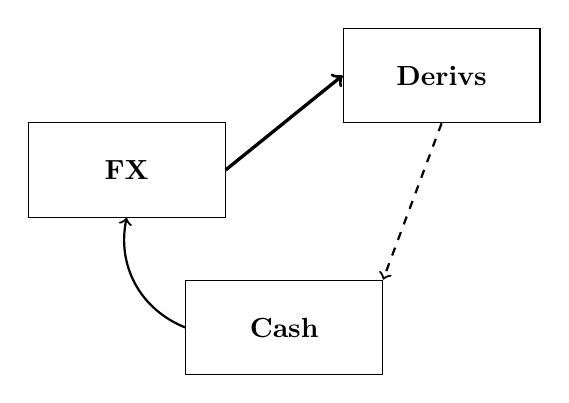
\begin{tikzpicture}[
      node distance=3cm,
      box/.style={draw, minimum width=2.5cm, minimum height=1.2cm, font=\bfseries, align=center},
      thickarrow/.style={->, line width=1.2pt},
      dashedarrow/.style={->, thick, dashed},
      curvedarrow/.style={->, thick, bend left=40}
    ]
    
    % Nodes
    \node[box] (fx) at (0,0) {FX};
    \node[box] (derivs) at (4,1.2) {Derivs};
    \node[box] (cash) at (2,-2) {Cash};
    
    % Arrows
    \draw[thickarrow] (fx.east) -- (derivs.west);
    \draw[dashedarrow] (derivs.south) -- (cash.north east);
    \draw[curvedarrow] (cash.west) to (fx.south);
    
    \end{tikzpicture}
    
    \vspace{1.5em}
    
    % Vertical Legend
    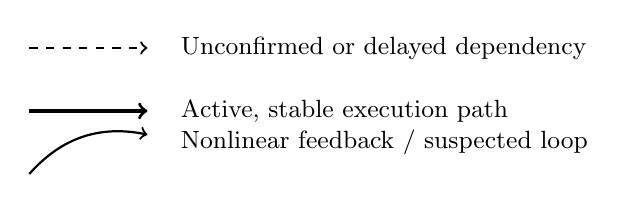
\begin{tikzpicture}[
      legend/.style={font=\small, anchor=west},
      dashsample/.style={->, thick, dashed},
      boldsample/.style={->, line width=1.2pt},
      curvesample/.style={->, thick, bend left=30}
    ]
    
    % Samples - vertical layout
    \draw[dashsample] (0,0) -- (1.5,0);
    \node[legend] at (1.8,0) {Unconfirmed or delayed dependency};
    
    \draw[boldsample] (0,-0.8) -- (1.5,-0.8);
    \node[legend] at (1.8,-0.8) {Active, stable execution path};
    
    \draw[curvesample] (0,-1.6) to (1.5,-1.1);
    \node[legend] at (1.8,-1.2) {Nonlinear feedback / suspected loop};
    
    \end{tikzpicture}
    
    \caption*{Legend: Arrow styles represent types of relationships between execution components.}
\end{figure}
    

\medskip

David had stood at the front and said:
“This is not a relay. It’s a choreography.”

“Then why not fire FX first?” someone had asked.
“Because FX moves before we do,” he replied. “If we hedge before the primary touches, we tell the 
street what we’re about to do.”

“And derivs?”

“They live in Chicago time. If we sync their clock to London, we break their book. If we don’t, 
we break ours.”

It had been one of those sessions — the kind where no one raised their voice because everyone 
understood the cost of being wrong.

What they had built wasn’t fragile, not exactly.
But it was threaded — stitched across markets like a pressure-sensitive suit.

Touch one panel wrong, and the whole garment wrinkles.
Touch it at the wrong time, and the seams tear.

Back then, someone from compliance had asked:
\textit{“What’s the fallback if one leg gets mispriced?”}

David didn’t blink.
“There isn’t one. That’s why we wait.”

Now, back in London, looking out over the city’s metal-glass silence,
he realized what the whole plan had always been:

Wait just long enough to be right.
But not so long that the market realizes you’re late.

Because latency isn’t just delay.
Latency is a window.
And if it closes on you mid-leg,
there’s no price in the book clean enough to fix it.





\subsection{What You Could Get Away With}


David nodded without looking up.
``Is the synthetic hedge platform fully deployed? I want confirmation we’re delta-matched and 
neutral on spread. No physical holds — just futures, options, or swaps as needed. If we’re going 
synthetic, it better rebalance fast enough to avoid slippage, and it better not light up 
compliance across venues.''

\medskip

\begin{TechnicalSidebar}{What is a Synthetic Hedge?}

  A \textbf{synthetic hedge} is a way to mimic the protective effect of a traditional hedge without 
  holding the actual asset.  
  Instead of directly owning the asset you want to protect --- like a stock or a commodity --- you 
  construct a position using financial derivatives such as:

  \medskip

  \begin{itemize}
    \item \textbf{Futures}: contracts to buy or sell an asset at a fixed price on a future date.  

    \medskip

    \textit{Example:} You agree today to buy 1,000 barrels of oil at \$80 per barrel, delivered three months from now — even if the market price changes in the meantime.

    \medskip
  
    \item \textbf{Options}: rights (but not obligations) to buy or sell at a specific strike price before a certain date.  

    \medskip

    \textit{Example:} You pay a small premium for the right to buy a stock at \$50. If it jumps to \$70, you profit. If it drops to \$30, you let the option expire and lose only the premium.

    \medskip
  
    \item \textbf{Swaps}: agreements to exchange cash flows tied to an asset’s performance, like interest rates or stock returns.  

    \medskip

    \textit{Example:} Two companies agree to swap payments: one pays based on a fixed 3\% interest rate, the other based on whatever LIBOR is. They do this to manage different funding risks.
  \end{itemize}
  

  \medskip

  These instruments allow you to \textit{replicate} exposure, neutralize risk, or generate offsetting returns (all without 
  touching the physical asset).

  \medskip

  Synthetic hedges are faster to deploy, easier to scale across jurisdictions, and often cheaper in terms of capital 
  or regulation. But they also come with trade-offs:

  \medskip

  \begin{itemize}
    \item \textbf{Increased model risk}: due to abstraction from underlying market mechanics.  

    \medskip
    \textit{Example:} Like using a flight simulator to train for real-world flying — if the simulator has bad settings, you won’t notice real turbulence until it’s too late.
    \medskip
  
    \item \textbf{Potential for hidden leverage}: small moves in the market can lead to outsized losses because you're controlling large exposures with minimal upfront cost.  
    \medskip
    \textit{Example:} It's like putting down a 5\% deposit to control a \$1 million house — if prices drop slightly, you could still lose everything.
    \medskip
  
    \item \textbf{Sensitivity to correlation assumptions and counterparty exposure}: synthetic hedges often rely on assets moving together in predictable ways, or on counterparties honoring deals.  
    \medskip
    \textit{Example:} Imagine buying flood insurance from a neighbor who also lives on the river. If the river floods, you both lose — and your “protection” might not show up.
  \end{itemize}
  

  \medskip

  In David’s case, the synthetic hedge platform meant Arcadia could rebalance across global venues without triggering 
  the same regulatory constraints, but it also meant any misalignment could propagate faster than legacy systems 
  could catch.

\end{TechnicalSidebar}

\medskip

``Yep. EU regulation’s lighter on delta thresholds. We have more elasticity on notional wraps,'' she said, 
scrolling through the live monitor.


\medskip

\begin{TechnicalSidebar}{What Are Delta Thresholds?}

  In trading, \textbf{delta} measures how much the value of a position changes in response to a change in the price 
  of the underlying asset.  
  A delta of 1.0 means a \$1 move in the asset causes a \$1 move in the position. A delta of 0.5 means only a \$0.50 
  move, and so on.

  \medskip

  \textbf{Delta thresholds} are regulatory or internal risk limits that restrict how much directional exposure a 
  portfolio or synthetic instrument can carry.  
  These thresholds are especially important for complex or leveraged positions, such as:

  \medskip

  \begin{itemize}
    \item \textbf{Derivatives with embedded leverage}: financial contracts that let you control a large position with a small upfront cost.  

    \medskip

    \textit{Example:} Like renting a Ferrari for the price of a scooter — you get speed and power, but if you crash, the bill is still full-sized.

    \medskip
  
    \item \textbf{Synthetic swaps or basket trades}: complex financial instruments that mimic the behavior of multiple underlying assets, often without holding any of them directly.  

    \medskip

    \textit{Example:} Like betting on the combined scores of five sports teams without watching any of the games — you win or lose based on an index you don’t actually control.

    \medskip
  
    \item \textbf{Algorithmically generated hedges}: risk protection strategies automatically built and adjusted by computer models, often in real time.  

    \medskip

    \textit{Example:} Like a self-driving car that constantly changes lanes to avoid traffic — fast and responsive, but if the sensors are off, it might drive straight into a wall.
  \end{itemize}
  

  \medskip

  Tighter delta thresholds mean tighter control — trades must stay close to neutral or hedged exposure.  
  Looser thresholds allow greater directional bets, larger notional swings, and more elasticity in how positions 
  are wrapped and deployed.

  \medskip

  In this case, EU regulation being “lighter on delta thresholds” means the model can take on more delta — more 
  market sensitivity —  
  without triggering a compliance block. It creates flexibility, but also introduces risk: the system can swing 
  wider before hitting a stop.

\end{TechnicalSidebar}

\medskip

``We’ve got no physical exposure on the books. All synthetic. Mix of short-dated futures for the front 
leg, plus some laddered calls in London and Frankfurt. The swaps desk’s holding neutral — delta-matched 
within 10 basis points. We set the auto-rebalance to trigger if correlation assumptions break outside 
tolerance.''

She looked up. ``No compliance flags so far. Liquidity bands holding. And if it moves too fast, we’ve 
got unwind logic pre-wired by venue.''
A pause. ``It’s quiet now, but the system’s listening.''

The words that landed were clean, confident, and factual.
But in his mind, they echoed with the ghost of a whiteboard marker squeaking on glass.

He was back in Luxembourg.

Not for the scenery. Not for the tax code — though that helped.

The meeting had to be there because that’s where the carve-out lived.
A bespoke entity, ring-fenced for jurisdictional flexibility and structured just thinly enough to avoid tripping oversight triggers in London or New York.

Luxembourg offered what the others couldn't:
\textit{neutrality without scrutiny.}
A sandbox for structured exposure.
A place where reporting thresholds were softer, risk categorization more pliable, and synthetic instruments could be tested just outside the perimeter of consolidated supervision.

The lawyers had called it “geo-optimization.”
The structurers called it “the buffer.”
David called it what it was: plausible deniability.

They didn’t bring full teams. Just enough people to call it a workshop.
Enough ambiguity to avoid board minutes, but enough technical clarity to push the boundary of the architecture.

They filled the whiteboard in layers — venue behavior, stress scenarios, cross-currency overlays.
But underneath it all was the same unspoken question:

What can we get away with… if the delta doesn’t spike?

That was the real reason they flew to Luxembourg.
Not for strategy.
But for insulation.
For a place to ask the wrong questions — and not be told no.

\medskip

\begin{HistoricalSidebar}{Why Luxembourg? A Soft-Law Capital for Hard-Money Games}

    Luxembourg may be smaller than Rhode Island, but in structured finance, size isn’t the metric that matters.

    \medskip
    
    What matters is architecture — legal, fiscal, and regulatory.
    
    \medskip
    
    Since the 1990s, Luxembourg has become a global hub for structured investment vehicles (SIVs), special purpose entities (SPEs), and cross-border funds. Not because it’s secretive in the Swiss sense, but because it offers a uniquely accommodating legal environment:

    \medskip
    
    \begin{itemize}
    \item \textbf{Flexible entity structures:} From the Société d’Investissement à Capital Variable (SICAV) to the newer RAIF (Reserved Alternative Investment Fund), Luxembourg lets you match your entity structure to your risk appetite.
    
    \item \textbf{Light-touch regulation:} Funds can operate under “passporting” rules via EU directives (like UCITS or AIFMD), but in practice, certain structures avoid full supervisory friction — especially if they’re not publicly distributed.
    
    \item \textbf{Tax efficiency without scandal:} Luxembourg isn’t a blacklisted tax haven. It’s OECD-compliant, but its double-tax treaties, thin-cap rules, and tolerance for hybrid instruments make it a favorite for optimizing exposure without lighting compliance alarms.
    \end{itemize}
    
    \medskip
    
    So why fly there?

    \medskip
    
    Because while the \textbf{war room is in New York}, the risk architecture is often offshore — not just in geography, but in logic.
    
    \medskip
    
    \begin{itemize}
    \item New York is where the trades happen.
    \item Luxembourg is where the liabilities sleep.
    \end{itemize}
    
    That’s why deal teams meet there.

    \medskip
    
    Not to decide strategy — but to shape the vessel that will carry it.

    \medskip
    
    In Luxembourg, conversations aren’t recorded. Term sheets are reviewed in person. And “structure” becomes a verb.
    
    \medskip
    
    It’s not about hiding. It’s about anchoring the legal fiction in the right jurisdiction.

    \medskip
    
    Because once the entity is domiciled, the map — and the rules — change.
    
\end{HistoricalSidebar}

\medskip

Not the conference room — the smaller one. The off-calendar prep call before the vendor roadshow.
Where the conversation hadn’t been about compliance. It had been about \textit{what you could get 
away with, if the delta didn’t spike}.

\textit{“We wrap it tight — low delta, small notional, but levered exposure.”}
That had been Sofia from structuring. Calm, like she was describing the weather.

\begin{TechnicalSidebar}{The Structuring Desk — Architects of Financial Engineering}

    In modern finance, the \textbf{structuring team} sits at the intersection of product design, 
    legal arbitrage, and quantitative engineering.
    
    They don’t pitch.  
    They don’t execute.  
    They build.
    
    \bigskip
    
    \textbf{What do they structure?}  
    Custom financial products — often bespoke derivatives, wrapped securities, or hybrid instruments 
    that don’t fit into clean categories.
    
    \begin{itemize}
      \item \textbf{Total Return Swaps (TRS)}
      \item \textbf{Synthetic ETFs}
      \item \textbf{Credit-Linked Notes (CLNs)}
      \item \textbf{Volatility-controlled wrappers}
    \end{itemize}
    
    \bigskip
    
    \textbf{Why does it matter?}
    
    Because structurers don’t just ask,  
    \begin{quote}
      \textit{“What’s the exposure?”}  
    \end{quote}
    They ask,  
    \begin{quote}
      While delivering the same risk,
      how can we wrap this exposure to satisfy compliance, balance sheet constraints, and 
      marketing optics?
    \end{quote}
    
    \bigskip
    
    \textbf{Three core mandates:}
    
    \begin{itemize}
      \item \textbf{Regulatory Awareness:}  
      Know the edge of the rulebook — and how to stay just inside it.
    
      \item \textbf{Risk Translation:}  
      Convert complex exposures into more palatable formats (e.g., lower delta, lower notional, higher leverage).
    
      \item \textbf{Sales Enablement:}  
      Make the exotic feel ordinary.  
      If a trader sells volatility, the structurer wraps it in something the client can understand — or legally hold.
    \end{itemize}
    
    \bigskip
    
    \textbf{A Structurer’s Motto (Unofficial):}  
    \begin{quote}
      “If you can’t move the risk, move the wrapper.”
    \end{quote}
    
    Which is why in prep calls and quiet rooms, the question isn’t “Is it compliant?”  
    It’s:  
    \begin{quote}
      \textit{“Can we show the optics without the spikes?”}
    \end{quote}
    
    Because in structured products, what’s \textbf{visible} often matters more than what’s \textbf{real}.
    

\end{TechnicalSidebar}

\medskip

Sophia let the words settle, then glanced around the room — not condescending, just aware that not 
everyone operated at her altitude.

“Just to level-set,” she said. “There are three ways to chase exposure. You can go high delta, high 
notional — that’s brute force. It tracks the underlying precisely, but it also triggers every compliance 
alert from here to Delaware.”

A few nods.

“Or you can go high notional, low delta — like macro overlays. Looks clean on paper but gets messy when 
rates shift or basis moves.”

She tapped the term sheet lightly.

“We choose the third lane: low delta, small notional, high leverage. That way the instruments don’t shout 
position. They whisper. You get the same directional profile without tripping any wires.”

\medskip


\begin{table}[H]
\centering
\caption{Comparison of Exposure Strategies}
\begin{tabularx}{\textwidth}{|X|X|X|X|}
\hline
\textbf{Strategy} & \textbf{Delta / Notional} & \textbf{Use Case} & \textbf{Trade-Offs} \\
\hline
\textbf{Brute Force} & High delta, high notional & Precise tracking of underlying asset & Full transparency, triggers compliance alerts \\
\hline
\textbf{Macro Overlay} & Low delta, high notional & Broad hedging or directional bias & Clean optics, but unstable if rates or basis shift \\
\hline
\textbf{Disclosure-Efficient} & Low delta, low notional, high leverage & Quiet directional exposure & Stays under radar, but needs constant monitoring and rebalancing \\
\hline
\end{tabularx}
\end{table}



\medskip








Someone asked — carefully, not confrontational —
“Don’t we need swap disclosure?”

It was Nathan — the junior from London, fresh off his Series 7 and still reading footnotes like they 
were commandments.

\medskip

\begin{TechnicalSidebar}{Swap Disclosure: What Must Be Reported, and When}

    Under U.S. financial regulation, \textbf{swaps} --- particularly \textbf{total return swaps (TRS)} and 
    other derivatives --- are subject to reporting requirements depending on their structure, counterparties, 
    and systemic risk potential.
    
    \medskip
    
    Key regulatory frameworks include:
    
    \medskip
    
    \begin{itemize}
      \item \textbf{Dodd-Frank Act} (2010): Requires many swaps to be reported to \textbf{Swap Data Repositories (SDRs)}.
      \item \textbf{SEC Rules 13D and 13G}: May trigger public disclosure if the swap gives beneficial ownership 
      or control over more than 5\% of a company's voting shares.
      \item \textbf{CFTC Reporting}: Mandates real-time and post-trade reporting of certain swap details (counterparty, 
      notional amount, pricing).
    \end{itemize}
    
    \medskip
    
    \textbf{However:} Disclosure may not be required if:

    
    \medskip
    
    \begin{itemize}
      \item The swap does not confer voting rights or control.
      \item The notional exposure remains below regulatory thresholds.
      \item The transaction is conducted through exempt counterparties or offshore entities.
    \end{itemize}
    
    \medskip
    
    \textbf{Layman Example:}  
    Imagine a hedge fund wants exposure to 4.9\% of a company’s stock without triggering public ownership filings.  
    Instead of buying shares directly, they enter a \textbf{total return swap} with a bank, which holds the shares 
    on its balance sheet.  
    The fund receives profits (or losses) as if it owned the shares — but since it technically doesn’t, no 13D 
    filing is required.  
    To the public, the fund appears uninvolved.  
    To the market, it's invisible.  
    But economically, it holds the same stake.
    
\end{TechnicalSidebar}

\medskip

Sofia didn’t flinch. She was smoothing her cuff, not even looking up from the term sheet.

“Not if the exposure stays within bounds,” she said calmly.

Nathan blinked. “But—sorry—aren’t swaps, like, reportable under Dodd-Frank? If we’re using them to 
replicate a position, isn’t that... material?”

She finally looked at him. Not annoyed. Not amused. Just… steady.

“Material to whom?” she asked. “The client? Compliance? The SEC?”

He hesitated. “Well... all of them?”

A few quiet chuckles around the table.

Sofia leaned back, folding her hands loosely.

“Okay, Nathan,” she said, “think of it like this. Let’s say you want to carry water across the border. 
Big jugs of water. But the customs limit says one liter per person.”

He nodded, still a little lost.

“So,” she continued, “you don’t bring one giant jug. You bring four friends. Everyone carries a liter. 
All within the limit. No flags raised.”

“That’s legal?”

She smiled faintly. “It’s within regulation. That’s the game.”

Nathan frowned. “But it’s still four liters of water.”

“Right,” she said. “But not in one container. Same with swaps. One big exposure triggers scrutiny. 
But split it — limit the notional, keep the delta low, rebalance frequently — and it stays under the 
radar.”

He leaned forward, trying to catch up. “So... it’s like smuggling, but politely?”

Sofia tilted her head. “It’s disclosure-efficient structuring.”

Someone else chimed in. “It’s not about hiding. It’s about not shouting.”

“And if the risk spikes?” Nathan asked.

“That’s what limits are for,” she said. “We pre-wire the unwind. We use triggers. If the exposure 
steps out of bounds, we step out of the position.”

He sat back, still chewing on the metaphor.

“You’re thinking in ethics,” she said gently. “We think in thresholds.”

And just like that, the meeting moved on.

\medskip

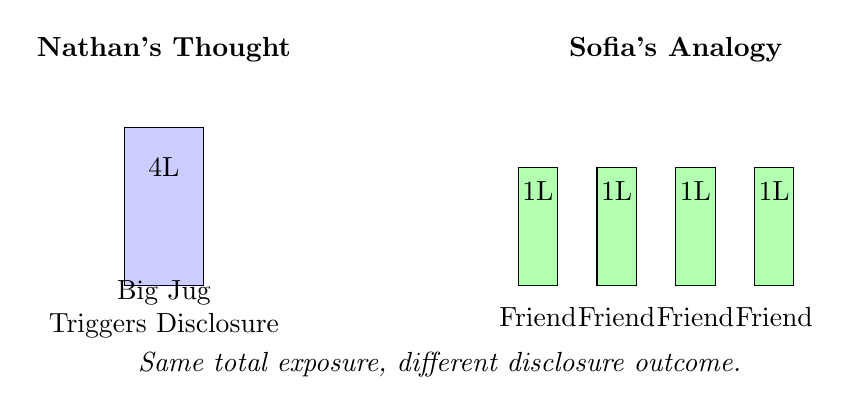
\begin{tikzpicture}

    % Title labels
    \node[align=center, font=\bfseries] at (1.5, 4) {Nathan's Thought};
    \node[align=center, font=\bfseries] at (8, 4) {Sofia's Analogy};
    
    % Nathan's Big Jug
    \draw[fill=blue!20, draw=black] (1,1) rectangle ++(1,2);
    \node at (1.5,2.5) {4L};
    \node[align=center] at (1.5,0.7) {Big Jug\\Triggers Disclosure};
    
    % Sofia's Small Jugs
    \foreach \i in {0,1,2,3} {
      \draw[fill=green!30, draw=black] (6+\i*1,1) rectangle ++(0.5,1.5);
      \node at (6.25+\i*1,2.2) {1L};
      \node[align=center] at (6.25+\i*1,0.6) {Friend};
    }
    
    % Caption
    \node[align=center, font=\itshape] at (5,0) 
      {Same total exposure, different disclosure outcome.};
    
\end{tikzpicture}

\medskip

\begin{HistoricalSidebar}{Dodd-Frank and the Illusion of Transparency}

    The \textbf{Dodd–Frank Wall Street Reform and Consumer Protection Act} was signed into law in 2010, 
    a sweeping response to the 2008 financial crisis. It promised accountability, oversight, and above 
    all: transparency.
    
    \medskip
    
    At its core, Dodd-Frank aimed to shine a light on the shadowy corners of finance — especially on 
    derivatives like \textbf{total return swaps}, \textbf{credit default swaps}, and other off-balance-sheet 
    magic tricks that helped implode global markets.
    
    \medskip
    
    Among its tools:

    \medskip
    
    
    \begin{itemize}
      \item \textbf{Title VII} regulated derivatives trading through central clearing and real-time reporting.
      \item \textbf{Section 13} (a.k.a. the Volcker Rule) restricted proprietary trading by banks.
      \item \textbf{Office of Financial Research (OFR)} was created to monitor systemic risk.
    \end{itemize}
    
    \medskip
    
    But as always, reform met reality.

    \medskip
   
    \begin{itemize}
        \item \textbf{Reporting thresholds were raised.}
        \item \textbf{Loopholes were rebranded as exemptions.}
        \item \textbf{Enforcement got outsourced to interpretation.}
    \end{itemize}
    
    \medskip
    
    Firms didn’t stop structuring risk.

    \medskip
    
    They just started calling it something else.
    
    \medskip
    
    By 2020, private funds had perfected the art of \textbf{economic exposure without legal ownership}. Swaps 
    became mirrors that let investors “replicate” positions without triggering disclosures meant for 
    actual shareholders.
    
    \medskip
    
    So yes, Dodd-Frank technically requires swap disclosure.

    \medskip
    
    But as Sofia understood — and Nathan was still learning — \textit{technicality is a poor substitute 
    for enforcement}.
    
\end{HistoricalSidebar}

\medskip

David had stared at the model on screen.
An options tree with synthetic deltas shaded like heat zones.

It was beautiful, in a terrifying way — a branching lattice of possibilities, each node a 
conditional future priced in microseconds.
The paler regions were low-risk: hedged, capped, buffered by structure.
But the deeper reds — they glowed like warning flares.

Those were the trades with teeth.
The ones with leverage baked in.
The ones that looked stable at the surface but spiked in exposure when the wind changed by 
half a basis point.

Each shade wasn’t just a number.
It was a bet.
A bet on volatility. On liquidity. On the assumption that nothing — not rates, not sentiment, 
not regulators — would move too fast.

He zoomed in. A single node, labeled 0.82 delta, flared crimson.
That one alone could tip the balance sheet if liquidity dried up.

The tree didn’t lie.
It just didn’t warn you when it was hungry.

David exhaled.
This wasn’t risk modeling anymore.
This was choreography — a delicate, probabilistic ballet performed on a stage where the floor might collapse without notice.

\medskip


\begin{figure}[H]
    \centering
    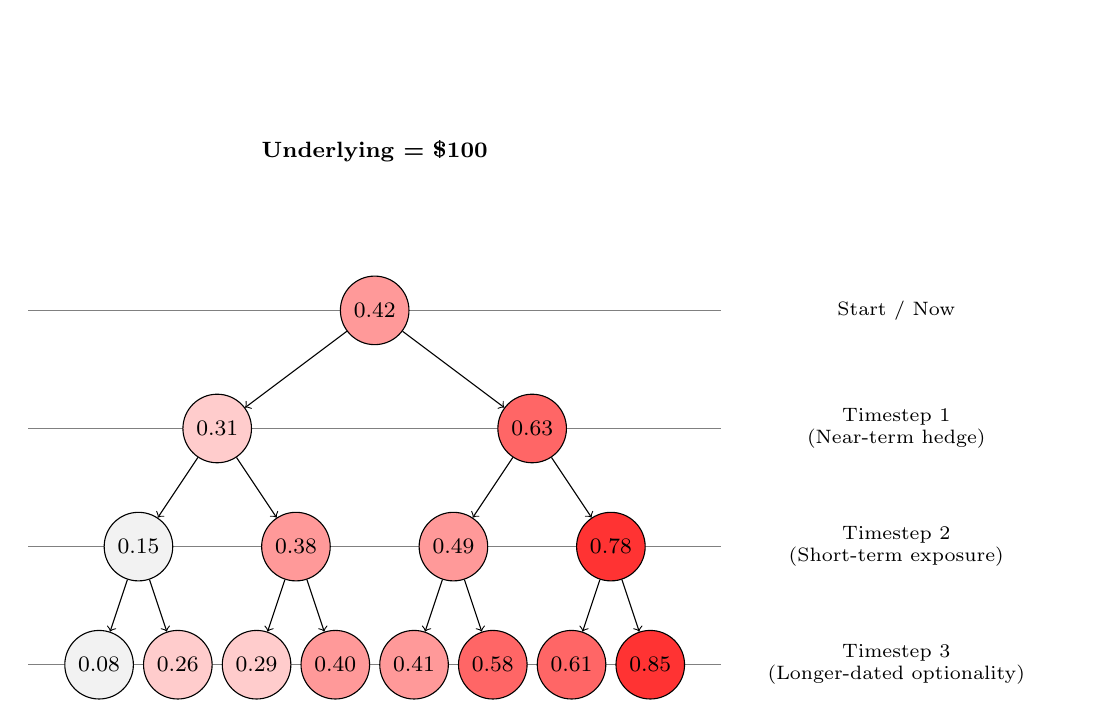
\begin{tikzpicture}[
        level distance=1.5cm,
        level 1/.style={sibling distance=4cm},
        level 2/.style={sibling distance=2cm},
        level 3/.style={sibling distance=1cm},
        every node/.style={circle, draw, minimum size=0.8cm, font=\footnotesize, text=black},
        edge from parent/.style={draw, ->}
      ]
  
      % Color definitions for synthetic deltas
      \tikzset{
        hot0/.style={fill=black!5},
        hot1/.style={fill=red!20},
        hot2/.style={fill=red!40},
        hot3/.style={fill=red!60},
        hot4/.style={fill=red!80}
      }

      \draw[solid, gray] (-4.4,0) -- (4.4,0) 
        node[right, font=\scriptsize, draw=none, fill=none, shape=rectangle] 
        {\parbox{4.2cm}{\centering Start / Now}};
      \draw[solid, gray] (-4.4,-1.5) -- (4.4,-1.5) 
        node[right, font=\scriptsize, draw=none, fill=none, shape=rectangle] 
        {\parbox{4.2cm}{\centering Timestep 1\\(Near-term hedge)}};
      \draw[solid, gray] (-4.4,-3) -- (4.4,-3) 
        node[right, font=\scriptsize, draw=none, fill=none, shape=rectangle] 
        {\parbox{4.2cm}{\centering Timestep 2\\ (Short-term exposure)}};
      \draw[solid, gray] (-4.4,-4.5) -- (4.4,-4.5) 
        node[right, font=\scriptsize, draw=none, fill=none, shape=rectangle] 
        {\parbox{4.2cm}{\centering Timestep 3\\ (Longer-dated optionality)}};
  
      % Tree definition with synthetic delta intensity
      \node[hot2, label=above:{\textbf{Underlying = \$100}}] {0.42}
        child {node[hot1] {0.31}
          child {node[hot0] {0.15}
            child {node[hot0] {0.08}}
            child {node[hot1] {0.26}}
          }
          child {node[hot2] {0.38}
            child {node[hot1] {0.29}}
            child {node[hot2] {0.40}}
          }
        }
        child {node[hot3] {0.63}
          child {node[hot2] {0.49}
            child {node[hot2] {0.41}}
            child {node[hot3] {0.58}}
          }
          child {node[hot4] {0.78}
            child {node[hot3] {0.61}}
            child {node[hot4] {0.85}}
          }
        };
  
    \end{tikzpicture}
  
    \vspace{1em}
  
    \begin{tabular}{|c|c|}
      \hline
      \textbf{Delta Range} & \textbf{Visual Cue / Interpretation} \\
      \hline
      $\delta < 0.2$ & \cellcolor{black!5} Lightest — Minimal directional sensitivity \\
      $0.2 \leq \delta < 0.4$ & \cellcolor{red!20} Low-moderate exposure \\
      $0.4 \leq \delta < 0.6$ & \cellcolor{red!40} Balanced option exposure \\
      $0.6 \leq \delta < 0.8$ & \cellcolor{red!60} High directional correlation \\
      $\delta \geq 0.8$ & \cellcolor{red!80} Near-linear tracking with underlying asset \\
      \hline
    \end{tabular}
  
    \caption{Options Tree Visualization with Time-Labeled Rows and Delta Intensity Heatmap}
\end{figure}



\medskip


He had asked:
“What's the elasticity look like under stress?”

Sofia:
\textit{“Better than real. Because we’re modeling control, not cash.”}

Someone else:
\textit{“If real hedges cost too much, synthetics give you a pass.”}

David remembered the way that felt. Not wrong — just fast.
A feeling that the trade wasn't being made. It was being described into existence.

He had said yes. Eventually.
Because when the desk asked for exposure without visibility,
synthetics were the answer that didn’t have to be explained in the audit notes —
only in the footnotes.

\medskip

Back in London now, he stared out over the skyline,
remembering how they’d phrased it:
\textit{“EU reg lets us flex the wrap.”}

Flex. Not “hedge.” Not “protect.”
Just... flex.

And he wondered, not for the first time,
if elasticity was just another word for a loophole
you haven't been caught using yet.


“And the latency?”

“Thirty-seven milliseconds desk to desk. Aurora’s already ported the model footprint to the London grid. 
Real-time sync across venues.”

\medskip

\begin{TechnicalSidebar}{Why Latency Matters in Trading}

  \textbf{Latency} refers to the delay between the moment a trading signal is generated and when it 
  is executed on an exchange.  
  In high-frequency and cross-venue trading, even a few milliseconds can mean the difference 
  between arbitrage and loss.

  \medskip

  \textbf{Thirty-seven milliseconds desk to desk} might sound fast, but in trading terms, it’s an eternity 
  compared to sub-millisecond co-located systems.  

  \medskip

  That latency includes:

  \begin{itemize}
    \item Signal generation and transmission
    \item Routing across network hops (e.g., New York to London)
    \item Exchange confirmation and roundtrip acknowledgment
  \end{itemize}

  \medskip

  \textbf{Porting the model to the London grid} means Aurora reduced some of that latency by 
  shifting compute closer to the venue.  
  Real-time synchronization across venues ensures consistency in state, but only if latency 
  is stable and predictable.

  \medskip

  In this case, 37ms is a performance ceiling.  
  It defines how reactive the system can be under stress, and how quickly risk can be 
  neutralized when the market turns.

\end{TechnicalSidebar}

\medskip

David leaned back, eyes scanning the floor. It looked calm.
It always did right before.




